\chapter[Алгоритмы генерации и обработки данных]{Алгоритмы генерации \\ и обработки данных} \label{chapt2}

В этой главе описываются постановки задач аппроксимации данных, а также исследованные алгоритмы генерации 
синтетических данных и
экстраполяции тарировочных данных. 


\section{Подходы к аппроксимации функций}\label{sect2_1}
% поправить слова
Метод наименьших квадратов --- один из базовых методов для оценки неизвестных 
параметров моделей по набору данных, при этом исследуется на минимум
следующая функция

\begin{equation}
\label{eq:square_minimum}
s(\vec{p}) = \frac{1}{2} \displaystyle \sum_{i=1}^N \phi_i(x, \vec{p})^2 , где
\end{equation}


%\begin{center}
% $ s(\vec{p}) = \left| f(x_t, \vec{p}) - y_t \right| ^ 2 \rightarrow min $
%\end{center}


$\vec{p}$ --- вектор оцениваемых параметров модели размерности $M$, $\phi_i(x,\vec{p}) = f(x_i, \vec{p}) - y_i $
--- функция, аппроксимирующая значения $y_i$ в точках $x_i$.

Во многих случаях существует аналитическое решение для системы $M$ уравнений 
$m \in [1..M]$
\begin{center}
 $ \displaystyle\sum_{i = 1}^N \left( y_i - f(x_i,\vec{p})\right) 
 \frac{\partial f(x_i, \vec{p})}{\partial p_m} = 0.$
\end{center}

\subsection{Постановка линейной задачи меньших квадратов}

Если зависимость модели от параметров $\vec{p}$ имеет вид 

\begin{center}
$ y_i = \displaystyle\sum_{j=1}^{M}p_j x_{ij} + \epsilon_i = 
\left(\vec{x_i}^T,\vec{p}\right) + \epsilon_i, $ 
\end{center}
 то такая задача называется линейной. Эта задача решается аналитически, 
её решение можно найти в книгах по статистике, например \cite{linnik}.



\subsection{Нелинейная задача наименьших квадратов}


В общем случае, решения системы дифференциальных уравнений нет и 
применяются численные методы решения оптимизационных задач, 
основанные на градиентном спуске.

% % %todo %s/Зюбина-Петухова/Метод наименьших гиперболизированных нелинейных  квадратов НГНК/gi
\subsection[Метод наименьших гиперболизированных \\нелинейных  квадратов]{Метод наименьших гиперболизированных \\ нелинейных  квадратов}
Известно, что  мягкое излучение поглощается в одном-двух метрах породы \cite{cosmicrays}, мягкое излучение обладает
меньшей проникающей способностью, чем мюоны, но при этом оказывает влияние на измерение (статистическая погрешность).
Поэтому измерения на небольших глубинах (до нескольких метров) должны меньше учитываться при тарировке. 
Напротив, ошибки на больших глубинах должны больше учитываться, поскольку значение интенсивности  меньше в разы
(в $e$ раз на 10 м. в. э.). Метод наименьших гиперболизированных нелинейных  квадратов (НГНК) построен с учетом замечаний, он минимизирует следующую функцию: 

\begin{center}
$s(\vec{p}) = \displaystyle\sum_{i=1}^N \left|
\frac{f(x_i, \vec{p}) - y_i}{\min(\left|f(x_i, \vec{p})\right|, \left|y_i\right|)}\right|^2 
\frac{100\%}{N} \rightarrow min$ %enum
 
\end{center}


\section[Постановка задачи аппроксимации тарировочных кривых]{Постановка задачи аппроксимации \\ тарировочных кривых}\label{sect2_2}

Качество обработки результатов измерения существенно влияет на погрешность
получаемых результатов, которая в первую очередь определяется
качеством восстановления зависимости интенсивности потока мюонов от глубины в м. в. э.

Тарировочные данные, полученные при получении тарировочной кривой на воде, 
показывают, что интенсивность потока мюонов падает монотонно с увеличением
глубины, а первая производная интенсивности монотонно возрастает 
от отрицательных значений к нулю. Используя решение 
однородного уравнения переноса, имеющего экспоненциальный характер, было решено
искать целевую функцию в виде суммы экспонент:
%todo ссылка ур-е переноса
\begin{equation}
  \label{eq:approximation}
  \mathit{ f(x)  = \displaystyle\sum_{j=1}^{M/2} a_j e^{-b_j x} , a_j \geq 0 , b_j \geq 0  }  
\end{equation}



% Критерии, кроме того нужно рассказать про non-liner aleast squares
Функция $f(x)$ --- сумма $M/2$ экспонент, каждая экспонента зависит от двух параметров $a_i$ и $b_i$, таким образом вектор аппроксимируемых параметров $\vec{p}$ обладает размерностью $M$.
В качестве критерия для оценки параметров аппроксимации была выбрана следующая норма по методу НГНК: 
\begin{equation}
	\label{eq:zuybin_petuhov}
	s(\vec{p}) = \displaystyle\sum_{i=1}^N \left|
	\frac{f(\vec{p}, x_i) - y_i}{\min(\left|f(\vec{p}, x_i)\right|, \left|y_i\right|)}\right|^2 
	\frac{100\%}{N} \rightarrow min %enum
\end{equation}

Данный критерий похож на взвешенную задачу наименьших квадратов 
нелинейных функций, в зарубежной литературе можно встретить название 
Weightened Non-Linear Least Squares Problem. Эта задача отличается
от задачи минимизации наименьших квадратов делителем зависящим от номера измерения: 
\begin{center}
$w(\vec{p}) = \displaystyle\sum_{i=1}^N \frac{\left|f(\vec{p}, x_i) - y_i\right|^2}{w_i} \rightarrow min$
\end{center}
Один из способов решения задачи --- взвешивание измерений, и  дальнейшее использование любого из существующих методов для нахождения 
наименьших квадратов нелинейных функций.Однако, поскольку в методе НГНК в знаменателе 
находится функция, зависящая от минимизируемых параметров, 
данный способ не работает. 

Упростим $k$-е слагаемое выражения (\ref{eq:zuybin_petuhov}), для краткости опустим постоянные множители $N$, $100\%$ : 

\begin{center}
 \large{$ \left|\frac{f(\vec{p}, x_k) - y_k}{min(\left|f(\vec{p}, x_k)\right|, \left|y_k\right|)}\right|^2 = \left\{ {
    \left| 1 - \frac{y_k}{f(\vec{p}, x_k)}\right|^2 , \left|f(\vec{p}, x_k)\right| < \left|y_k\right|  \atop 
    \left| 1 - \frac{f(\vec{p}, x_k)}{y_k}\right|^2 , \left|f(\vec{p}, x_k)\right| > \left|y_k\right|  
 } \right. $}
\end{center}

Таким образом, разбивая $ M $--мерное пространство вектора параметров $ \vec{p}$ на две области, мы можем сформулировать 
критерий в терминах задачи наименьших квадратов нелинейных функций.
Рассмотрим кусочно-гладкую функцию $\psi_k(\vec{p}, x_k)$: 
\begin{center}
\large{$\psi_k(\vec{p}, x_k) = \left\{ {
    \frac{y_k}{f(\vec{p}, x_k)} , f(\vec{p}, x_k) < y_k  \atop 
    \frac{f(\vec{p}, x_k)}{y_k} , f(\vec{p}, x_k) > y_k  
 } \right.$}
\end{center}

Решая задачу о наименьших квадратах для функции 
$\psi(\vec{p}, \vec{x})$ на постоянном векторе данных, заполненным
единицами получаем решение для минимизации по методу НГНК, используя стандартные методы: 
$v(\vec{p}, \vec{x}) = \displaystyle\sum_{k=1}^N \left|1 -
\psi_k(\vec{p}, x_k)\right|^2 \rightarrow min$


\section{Генерация синтетических данных}\label{sect2_3}


Получение большого набора тестовых измерений (исходных данных 
для тарировочных кривых) сопряжено с рядом трудностей. Поскольку 
плотномер находится в активной разработке,
большую часть времени прибор недоступен для проведения тестовых
измерений. Кроме того, примерное время серии измерений составляет
около часа. Соответственно, для получения большего набора данных, время пропорционально растёт.


Ввиду перечисленных сложностей, предложено в качестве тестовых
данных для алгоритмов использовать синтетические данные. Было 
рассмотрено два подхода моделирования данных -- 
полная симуляция потока мюонов и генерация зашумленных данных 
на основе известной целевой функции (суммы монотонно убывающих экспонент).


\subsection{Программный пакет MUSIC}\label{subsect2_3_1}

%todo ссылки
В рамках работы был исследован ряд статей и монографий описывающих подходы и существующие
решения по моделированию мюонов. В результате в качестве ПО для 
генерации потока мюонов
был выбран программный пакет MUSIC (MUon SImulation Code). Он обладает
рядом достоинств --- 
%тут надо поправить текст/найти индекс цитирования
результаты его моделирования находятся в соответствии с экспериментальными
данными в широкой области энергий от нескольких ГэВ до 1 ТэВ (тогда, как ряд
%todo ссылка кочанов
моделей обладают
недостатком мюонов в определенных областях энергий). Данный программный 
пакет доступен бесплатно, доступен его исходный код, автор пакета
Кудрявцев В. А. \cite{kudryavcev} дал несколько 
советов по моделированию потока мюонов в среде.


Программный пакет MUSIC проводит моделирование в 3х измерениях с помощью 
метода Монте-Карло. Взаимодействие мюонов с материей с высокими
потерями энергии рассматриваются как стохастические процессы. При этом учитываются угловое отклонение 
и смещение мюонов из-за множественного рассеяния на ядрах атомов, 
потери энергии на тормозное излучение
и неупругое рассеяние. В данной работе для каждого тестового измерения 
проводилась симуляция 5000 мюонов и из статистики определялась вероятность
выживания мюонов на заданной глубине. 
Для тестирования алгоритмов было проведено 34 серии измерений по 10 измерений в серии. 


\subsection{Генерация данных на основе целевой функции}\label{subsect2_3_2}


Проверка алгоритмов на основе симуляции потока мюонов обладает 
одним недостатком --- неизвестна зависимость флуктуаций от  
кривой зависимости интенсивности 
потока мюонов от глубины. По этой причине была проведена другая серия 
синтетических измерений. В этой серии из допустимого диапазона 
параметров случайно определялись параметры 
экспонент, определялся "поток мюонов" на глубине и затем к этим 
данным добавлялся шум в пределах 5\% относительной погрешности.



\section{Алгоритмы экстраполяции тарировочной кривой}\label{sect2_4}

В ходе работы были рассмотрены следующие алгоритмы:

\begin{itemize}
 \item Прони-подобные алгоритмы
 \item Алгоритм Левенберга-Марквардта
 \item Модификация жадного алгоритма
 
\end{itemize}

Описание алгоритмов дается в соответствующих секциях

\subsection{Алгоритм Прони}\label{subsect2_4_1}

Алгоритм Прони был разработан Гаспаром Рише де Прони в 1795 году\cite{prony}. Чаще всего этот метод рассматривается в 
качестве метода анализа сигналов (выделения экспоненциально-затухающих
синусоидальных гармоник), но также может применяться и в других областях, например, при определении количества 
вещества в фармакинетике \cite{pharmakinetics}.

Подход метода Прони - в преобразовании экспоненциальных выражений к нелинейной алгебраической системе уравнений и 
дальнейшем преобразовании их в большее количество линейных алгебраических уравнений, которые могут быть решены 
методом наименьших квадратов. В предположении, что данные аппроксимируются суммой экспонент с M неизвестными

\begin{equation}
  \tag{\ref{eq:approximation}}
  \mathit{ f(x)  = \displaystyle\sum_{j=1}^{M/2} a_j e^{-b_j x} }.  
\end{equation}

Пусть $\mu_j = exp(-b_j)$, тогда выражение (\ref{eq:approximation}) можно представить в виде :

\begin{equation}
  \label{eq:prony_nonlinear}
  \mathit{ f(x)  = a_1 \mu_1^x + a_1 \mu_0^x + \ldots + a_M \mu_M^x }.
\end{equation}


Метод Прони накладывает дополнительные ограничения на измерение данных --- данные должны измеряться с равными 
интервалами и количество точек измерений $N \geq M$. В общем случае абсциссы данных перенормируются $x \to k = 0 \ldots N-1$, 
в случае с экспериментальными данными мюонного плотномера перенормировка не требуется, т. к. измерения на воде
проводятся каждый метр, начиная от уровня поверхности воды (нулевая глубина). После подстановки получаем:

\begin{equation}
  \begin{split}
  f_1  \approx a_1 \mu_1^0 + a_2 & \mu_2^0 + \ldots + a_{M/2} \mu_{M/2}^0; \\
  f_1  \approx a_1 \mu_1^1 + a_2 & \mu_2^1 + \ldots + a_{M/2} \mu_{M/2}^1;  \\
  f_2  \approx a_1 \mu_1^2 + a_2 & \mu_2^2 + \ldots + a_{M/2} \mu_{M/2}^2;  \\
  \vdots & \\
  f_N \approx a_1 \mu_{1}^{N-1} + a_2 & \mu_{2}^{N-1} + \ldots + a_{M/2} \mu_{M/2}^{N-1}.
  \end{split}
  \label{eq:prony_system}
\end{equation}

Для разрешения этой нелинейной системы алгебраических уравнений, введем временную переменную $\mu$ и составим уравнение: 

\begin{equation}
\label{eq:prony_algebra}
	\left( \mu - \mu_1 \right) 
	\left( \mu - \mu_2 \right) \cdots 
	\left( \mu - \mu_{M/2} \right) = 0, 
\end{equation}
$\mu_1,\mu_2, \ldots , \mu_{M/2}$ --- корни алгебраического
уравнения 

\begin{equation}
	\label{eq:prony_alpha}
	\alpha_0 \mu ^ {M/2} + 
	\alpha_1 \mu ^ {M/2-1} + 
	\alpha_2 \mu ^ {M/2-2} + \ldots
	\alpha_{M/2-1} \mu ^ 1 + 
	\alpha_{M/2} \mu ^ 0 = 0.
\end{equation}

В уравнении (\ref{eq:prony_alpha}) коэффициенты $\alpha_i = f (\mu_1, \mu_2, ... \mu_{M/2} )$  
--- неизвестные, их можно получить из системы $ N - M/2 $ уравнений

\begin{equation}
  \begin{split}
  f_{M/2} \alpha_0 + f_{M/2-1} \alpha_1 + f_{M/2-2} & \alpha_2 + \ldots + f_0 \alpha_{M/2} \approx 0;  \\
  f_{M/2+1} \alpha_0 + f_{M/2} \alpha_1 + f_{M/2-1} & \alpha_2 + \ldots + f_1 \alpha_{M/2} \approx 0; \\
  \vdots & \\
  f_{N-1} \alpha_0 + f_{N-2} \alpha_1 + f_{N-3} & \alpha_2 + \ldots + f_{N-M/2-1} \alpha_{M/2} \approx 0.  \\
  \end{split}
  \label{eq:prony_system2}
\end{equation}

Значения $f_i$ определены из результатов измерений, и поскольку \\ $N \geq M$, данная система является переопределенной линейной системой уравнений.


После определения коэффициентов $\alpha_i$, коэффициенты $\mu_i$ (и соответствующие им коэффициенты $b_i$) находятся
 как корни полинома (\ref{eq:prony_nonlinear}). После подстановки коэффициентов $\mu_i$ в (\ref{eq:prony_system}) получаем еще одну переопределенную линейную систему с неизвестными коэффициентами $a_1, a_1, \ldots, a_{M/2}$, которую
 также можно разрешить с помощью метода наименьших квадратов.  


Данный алгоритм имеет следующие модифакции --- Алгоритмы Кунга, Зейгера-МакЕвена, Осборна \cite{kung, zeiger, osborn}, которые были реализованы на языке octave и протестированы на экспериментальных и синтетических данных вместе с оригинальным алгоритмом. В результатах при аппроксимации двумя и более экспонентами при решении полинома (\ref{eq:prony_nonlinear}) возникают комплексные $\mu_i$, которым соответствуют синусоидальные гармоники, что противоречит физической модели измерения. 

По этой причине, в дальнейшем, данное семейство алгоритмов не рассматривается.




\subsection{Модификация жадного алгоритма}\label{subsect2_3_4}

Аппроксимация проводится в два этапа. На первом этапе находятся базовые экспоненты интерполяции. Поиск базовых экспонент  проводится перебором настроечного $\delta$ -- параметра, начиная с экспоненты с наименьшим значением $b_i$. Экспонента строится по двум точкам, так, чтобы она проходила через крайнюю правую тарировочную точку ($x_{j}, y_{j}$) и точку, расположенную ниже следующей тарировочной точки ($x_{j-1}, y_{j-1}$) на величину, задаваемую настроечным $\delta$-параметром. Если коэффициенты $a_i, b_i$ удовлетворяют условию (\ref{eq:approximation}), то найденная экспонента вычитается из исходной кривой. Если значения полученной кривой положительны, то для нее запускается новая итерация. В противном случае найденная экспонента бракуется и делается новая попытка построить экспоненту, но уже с использованием следующей точки ($x_{j-2}, y_{j-2}$). После завершения процедуры, для оценки вектора параметров применяется метод НГНК (\ref{eq:zuybin_petuhov}). В случае нахождения нового минимума решение фиксируется. Решение ищется
для $\delta$-параметра, лежащего в диапазоне $\left[\delta_{min};\delta_{max}\right]$.
\begin{figure} 
  \center
  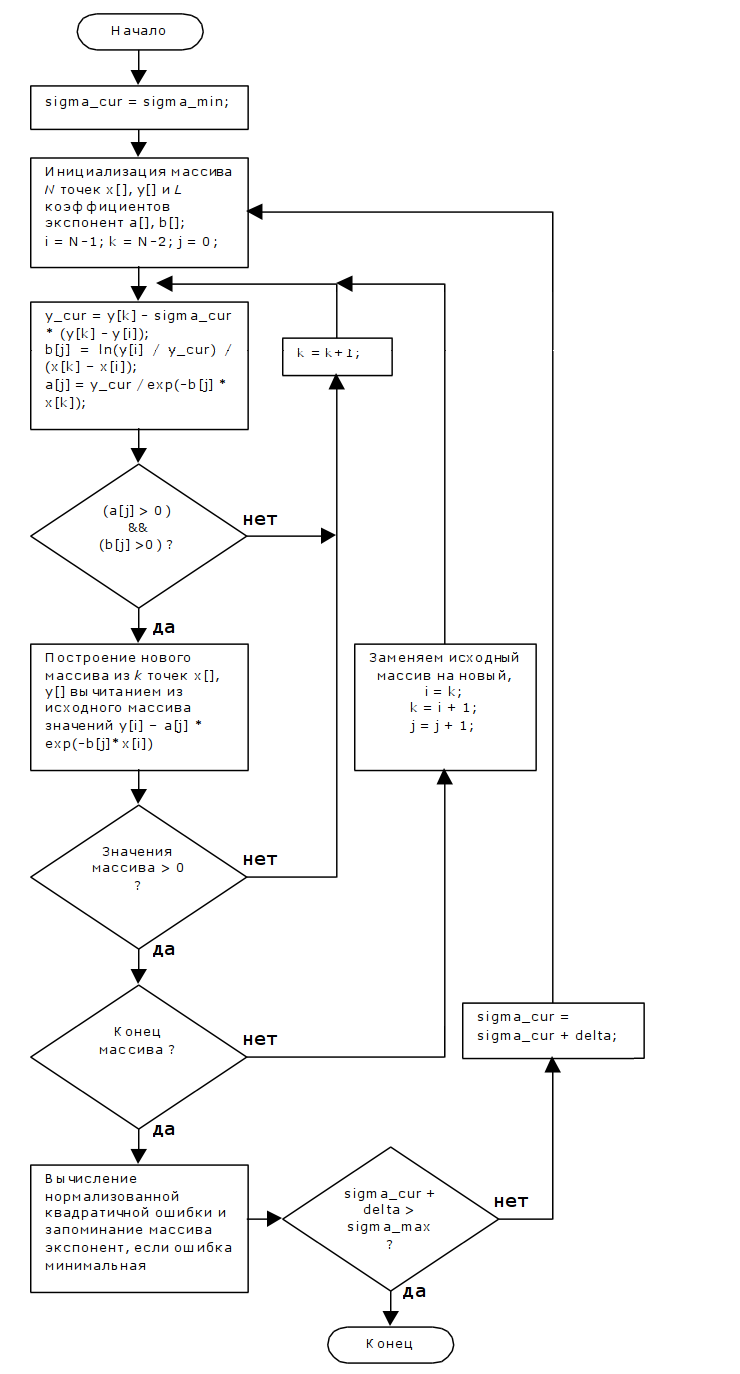
\includegraphics [scale=0.67] {greedy_schema}
  \caption{Блок-схема жадного алгоритма} 
  \label{img:greedy_schema} 

\end{figure}
На втором этапе проводится оптимизация степенных коэффициентов, найденных экспонент. Как и на первом этапе, оптимизация проводится по методу НГНК.

Подробнее работа алгоритма изображена на блок-схеме  (рис. \ref{img:greedy_schema})


\subsection{Алгоритм Левенберга-Марквардта}\label{subsect2_4_4}

Алгоритм Левенберга-Марквардта используется для оптимизации функций вида:

\begin{equation}
\tag{\ref{eq:square_minimum}}
F(\vec{p}) = \frac{1}{2} \displaystyle \sum_{i=1}^N \phi_i(\vec{p})^2,
\end{equation}
при этом используется алгоритм градиентного спуска:

\begin{enumerate}
 \item Задается начальное приближение $\vec{p_0}$ и точность рассчета $\epsilon$;
 \item Рассчитывается $ \vec{p_{i+1}} =  \vec{p_{i}} - \gamma \nabla F(\vec{p_{i}}) $;
 \item Проверяются условия $\left| \vec{p_{i+1}} - \vec{p_{i}} \right| > \epsilon, \left| F(\vec{p_{i+1}}) - F(\vec{p_{i}}) \right| > \epsilon $ если условия верны, то $i = i + 1$ 
 и выполняется шаг 2, иначе итоговый вектор $ \vec{p} = \vec{p_{i+1}} $.
\end{enumerate}
%особый вид матрицы Гессе.
Обозначим через $J(\vec{p}) m \times n$-матрицу Якоби для $f(\vec{p})$ и пусть $G_i(\vec{p})$ --- 
матрица Гессе для $f_i(\vec{p})$. Тогда выражения для градиента $g(\vec{p})$ и матрицы Гессе $G(\vec{p})$ функции
(\ref{eq:square_minimum}) будут выглядеть следующим образом:
\begin{equation}
\begin{split}
 g(\vec{p}) &= J(\vec{p})^T f(\vec{p}); \\
 G(\vec{p}) &= J(\vec{p})^T J(\vec{p}) + \displaystyle \sum_{i=1}^M f_i(\vec{p}) G_i(\vec{p}).
\end{split}
 \label{eq:levenberg_gesse}
\end{equation}
% Отсюда видно, что элементы $G(x)$  образованы комбинациями первых и вторых 
%производных функций $f_i$
%todo ньютоновская система.
Обозначим через $\vec{p}_k$ текущую оценку решения задачи минимизации функции (\ref{eq:square_minimum}),
тогда ньютоновская система в силу (\ref{eq:levenberg_gesse}) примет вид:
\begin{equation}
 \left(J^T_k J_k + Q_k\right) \vec{\tau}_k = -J^T_k f_k.
\end{equation}
Её решением будет вектор $\vec{\tau}_N$ --- ньютоновское направление. В случае алгоритма Ньютона-Гаусса, оно аппроксимируется  решением системы 
\begin{equation}
 (J^T_k J_k ) \vec{\tau}_k = -J^T_k f_k.
\end{equation}
Данная задача разрешима и включает только первые производные от $f$.

В алгоритме Левенберга-Марквардта направление поиска 
определяется, как решение системы уравнений вида:

\begin{equation}
 (J^T_k J_k + \lambda_k I) \vec{\tau}_k = -J^T_k f_k,
\end{equation}
$\lambda_k$ - некоторое неотрицательное число. В этом методе шаг вдоль $\vec{\tau}_k$ всегда 
полагается единичным, т.е. очередная точка $\vec{p}_{k+1} = \vec{p}_k + \vec{\tau}_k$. Монотонное убывание минимизируемой
функции достигается за счет подбора <<хороших>> значений $\lambda_k$. При $\lambda_k = 0$, направление будет 
направлением Гаусса-Ньютона, когда $\lambda_k \to \infty$ норма $\vec{\tau}_k$ стремится к нулю, и вектор
$\vec{\tau}_k$ в пределе становится параллельным антиградиенту. Неравенство $F (\vec{p}_k + \vec{\tau}_k) < F_k$ можно обеспечить
выбрав $\lambda_k$ достаточно большим. Однако при этом теряется информация о кривизне, и проявляются
недостатки метода градиентного спуска --- в места пологого наклона необходимо делать большие шаги, чем в случае
с крутым наклоном. Марквардт ввел модификацию в алгоритм Левенберга, учитывающую кривизну

\begin{equation}
 \left(J^T_k J_k + \lambda_k diag \lbrace J^T(\vec{p}) J(\vec{p} \rbrace \right) \vec{\tau}_k = -J^T_k f_k.
\end{equation}

Затем с вектором $\vec{\tau}_N$ проводится процедура градиентного спуска.

Главный недостаток алгоритма Левенберга-Марквардта --- сильная 
зависимость результатов от начальной оценки параметров $\vec{p_{0}}$. В итоговом алгоритме в 
качестве начальных оценок используются результаты работы метода перебора параметров 
аппроксимации и результаты модифицированного жадного алгоритма.

%todo Модифицированный алгоритм Левенберга-Марквардта

\subsection{Тестирование алгоритмов}
Исследованные алгоритмы были реализованы на языках octave (Левенберг-Марквардт, Прони), С++ (Численный перебор параметров),
 LabVIEW (модификация жадного алгоритма). Алгоритмы были протестированы на 68 сериях измерений по 10 измерений в каждой серии.
 34 серии были сгенерированы с помощью метода Монте-Карло, 34 с помощью генерации на основе известных целевых функций с добавлением шума. 
\begin{figure}[t]
  \begin{adjustbox}{addcode={\begin{minipage}{\width}}{\caption{%
      Результаты тестирования на алгоритмах
      }\label{img:generated_exp_data} \end{minipage}},rotate=90,center}

\begin{tikzpicture}
    \begin{axis}[ % начать график
        xlabel=Номер серии измерений, % метка для оси x
        ylabel=Значение ошибки по НГНК \%, % метка для оси y
        xtick align=center, % риски оси x внутри графика
        yminorgrids, ymajorgrids, % линии для основных и второстепенных значений по оси y
        xmajorgrids, % линии для основных значений по оси x
        minor y tick num=1, % 4 второстепенных риски между каждыми основными рисками по оси y
        width=25cm,
        height=17cm,
        %legend style={at={(0.70,0.64)}, anchor=south west} % позиционирование легенды относительно нижнего левого угла
    ],
        \addplot[black,mark=asterisk,style=solid] table[x=x,y=original] from {data/plot.dat}; % тёмно-зелёным отметить данные из столбца 'a' на оси таблицы midvalues 
        \addlegendentry{ORG} % добавить линию на легенду
        \addplot[black,mark=square*,style=dotted] table[x=x,y=mesh] from {data/plot.dat}; % тёмно-красным отметить на оси y данные из столбца 'b' таблицы midvalues 
        \addlegendentry{MSH} % добавить линию на легенду
        \addplot[gray,mark=diamond*,style=solid] table[x=x,y=leiserson] from {data/plot.dat}; % тёмно-жёлтым отметить на оси y данные из столбца 'c' таблицы midvalues 
        \addlegendentry{LMM} % добавить линию на легенду
        \addplot[black,mark=oplus*,style=dashed] table[x=x,y=greedy] from {data/plot.dat}; % тёмно-синей сглаженной линией отметить на оси y данные из столбца 'mid' таблицы midvalues 
        \addlegendentry{GD} % добавить линию на легенду
    \end{axis}
\end{tikzpicture}
  \end{adjustbox}
\end{figure}

\clearpage



Используемые сокращения: Модификация жадного алгоритма (GD), Левенберг-Марквардт (LM), Левенберг-Марквардт, модифицированный для использования в качестве оценки метод НГНК (LMM), численный перебор параметров экспонент (MSH), значение шума по методу НГНК на генерируемых данных (в случае с известной целевой функции) (ORG). 

Результаты тестирования представлены на графике (рис. \ref{img:generated_exp_data})






На данном графике по оси абсцисс отображены номера серий измерений (от 0 до 33), по оси ординат --- значения ошибок результатов аппроксимации по методу НГНК.

На таблице \ref{tab:expresults} приведены результаты тестирования алгоритмов на синтетических данных. В таблице перечислены минимальные, максимальные и среднее значение ошибки по методу НГНК на сериях по 34 измерения. 

% % ТАБЛИЦА


\begin{table}[h]
\centering
\caption{Результаты тестирования}
\pgfplotstabletypeset[
columns={alg, expavg, expmin, expmax, monavg, monmin, monmax},
columns/alg/.style={column name = Алгоритм, column type=|c|, string type}, 
columns/expavg/.style={column name = Avg, column type=|c},
columns/expmin/.style={column name = Min, column type=|c},
columns/expmax/.style={column name = Max, column type=|c|},
columns/monavg/.style={column name = Avg, column type=|c},
columns/monmin/.style={column name = Min, column type=|c},
columns/monmax/.style={column name = Max, column type=|c|},
every head row/.style={ before row={ %
\toprule %
\hline
& \multicolumn{3}{c||}{Целевая функция} & \multicolumn{3}{c|}{Метод Монте-Карло} \\ \hline 
},
after row={\midrule\hline}},
every last row/.style={ after row=\hline},
every first column/.style={ column type/.add={|}{|}},
every last column/.style={ column type/.add={}{|}}
]{data/expresults.dat}
	  
\label{tab:expresults}
\end{table}

%todo h2o markwardt graph modified diagramm


На уровне около 2\% находится график оригинальных экспонент без шума. В среднем, алгоритм Левенберга-Марквардта 
получает результат лучший, чем оригинальные экспоненты, однако в некоторых точках перебор параметров и модификация
 жадного алгоритма показывают меньшую погрешность. По этой причине был предложен и реализован комбинированный алгоритм.

\clearpage
\subsection{Комбинированный алгоритм}\label{sect2_4_5}

Предложенный комбинированный алгоритм состоит из двух частей: 

В первой части вычисляются начальные оценки $a_i, b_i$ параметров экспонент с помощью численного перебора и модификации жадного алгоритма. 
Далее вычисленные значения передаются в качестве первичных оценок в алгоритм Левенберга-Марквардта
 и модифицированный алгоритм Левенберга-Марквардта. Затем, из первичных оценок и результатов работы алгоритмов
 выбираются параметры экспонент, на которых норма (\ref{eq:zuybin_petuhov}) принимает минимальное значение,
 эти параметры возвращаются в качестве результата работы алгоритма  (рис. \ref{img:combined_algorithm}).
\begin{figure} [h]
\begin{tikzpicture}[thick, node distance=2.7cm, text height=1.5ex, text depth=.25ex, auto]
\node[datum] (data) {Данные};
\node[algorithm,below right of=data] (levenbergm)  {LMM};
\node[algorithm,right of=levenbergm]  (greedy) {GD};
\node[algorithm,right of=greedy] (levenberg) {LM};
\node[algorithm,below left of=data] (levenberg2) {LM};
\node[algorithm,left of=levenberg2]  (count) {MSH};
\node[algorithm,left of=count] (levenbergm2)  {LMM};
\node[algorithm,below left of=levenbergm]   (minimum) {Минимум};
\node[datum,below of=minimum]   (result){Результат};

\path[->,draw,>=latex',line width=3pt] (data) -- +(1,0) -| (greedy);
\path[->,draw,>=latex',line width=3pt] (data) -- +(-1,0) -| (count);
\path[->,>=latex',line width=3pt] (greedy) edge node {}(levenbergm);
\path[->,>=latex',line width=3pt] (greedy)  edge node {} (levenberg);
\path[->,>=latex',line width=3pt] (count) edge node {} (levenberg2);
\path[->,>=latex',line width=3pt] (count) edge node {} (levenbergm2);
\path[->,draw,>=latex',line width=3pt] (data)-- +(4.59,0) -- (levenberg);
\path[->,draw,>=latex',line width=3pt] (data)-- +(4.59,0) -- (levenbergm);
\path[->,draw,>=latex',line width=3pt] (data)-- +(-4.59,0) -- (levenberg2);
\path[->,draw,>=latex',line width=3pt] (data)-- +(-4.59,0) -- (levenbergm2);
\path[->,>=latex',line width=3pt] (greedy)  edge node {} (minimum);
\path[->,>=latex',line width=3pt] (count) edge node {} (minimum);
\path[->,draw,>=latex',line width=3pt] (levenberg) -- +(-2.8,-1.899) --  (minimum);
\path[->,>=latex',line width=3pt] (levenberg2) edge node {} (minimum);
\path[->,>=latex',line width=3pt] (levenbergm) edge node {} (minimum);
\path[->,draw,>=latex',line width=3pt] (levenbergm2) -- +(2.8,-1.899) --  (minimum);
\path[->,draw,>=latex',line width=3pt] (minimum) -- +(0, -0.5) -- (result);

\end{tikzpicture}
\center
\caption{Схема комбинированного алгоритма} 
\label{img:combined_algorithm} 
\end{figure}

\begin{figure} [h]
\begin{tikzpicture}[thick, node distance=2.7cm, text height=1.5ex, text depth=.25ex, auto]
\node[datum] (data) {Данные тарировки};
\node[algorithm,below of=data] (alg)  {Комбинированный алгоритм};
\node[datum,below of=alg]  (curve) {Тарировочная кривая};
\node[algorithm,left=4cm of alg] (interface) {Интерфейс оператора};
\node[datum,below of=interface] (data2) {Данные измерения};
\node[datum,below of=data2] (xo) {Радиационная длина};
\node[datum,below of=xo] (moisture) {Влажность};
\node[datum, below of=curve]   (density) {Плотность};

\path[->,>=latex',line width=3.5pt] (interface) edge node {} (data);
\path[->,>=latex',line width=3.5pt] (interface) edge node {} (alg);
\path[->,>=latex',line width=3.5pt] (curve) edge node {} (interface);
\path[->,draw,>=latex',line width=3.5pt] (interface) -- +(-3.5,-0) -- +(-3.5,-2.8) -- (data2);
\path[->,draw,>=latex',line width=3.5pt] (interface) -- +(-3.5,-0) -- +(-3.5,-5.4) -- (xo);
\path[->,draw,>=latex',line width=3.5pt] (interface) -- +(-3.5,-0) -- +(-3.5,-8.1) -- (moisture);
\path[->,>=latex',line width=3.5pt] (data) edge node {} (alg);
\path[->,>=latex',line width=3.5pt] (alg) edge node {} (curve);

\path[->,>=latex',line width=3.5pt] (xo) edge node {} (density);
\path[->,draw,>=latex',line width=3.5pt] (data2) -- (density); %-- +(3.5,0) -- +(3.5,-2.3) -- +(8, -2.3) 
\path[->,draw,>=latex',line width=3.5pt] (moisture)  -- (density); %-- +(3.5,0) -- +(3.5,2.3) -- +(8, 2.3)
\path[->,>=latex',line width=3.5pt] (curve) edge node {} (density);
\end{tikzpicture}
\center
\caption{Схема комбинированного алгоритма} 
\label{img:combined_algorithm} 
\end{figure}

\section[Архитектура системы автоматизации обработки данных]{Архитектура системы автоматизации \\ обработки данных}\label{subsect2_5}

На данный момент измерительная система состоит из погружаемой части плотномера, блока управления и АРМ оператора. Измерительная часть плотномера состоит из металлического кожуха, сцинтиллятора, фото-электронного умножителя и усилителя сигнала, соединенного посредством длинной линии с блоком управления. В блоке управления плотномером находится кнопка запуска/сброса, встроенный таймер на 5 минут и счетчик мюонов с дисплеем.

Оператор системы собирает показания прибора и сохраняет их в файл, который передается на АРМ оператора. АРМ оператора --- программный комплекс, установленный стационарном или мобильном компьютере. АРМ имеет два режима работы --- режим тарировки, в котором доступны следующие операции:

\begin{enumerate}
	\item Загрузка/модификация тарировочных данных;
	\item Построение тарировочной кривой;
	\item Ручная подстройка параметров;
	\item Сохранение тарировочной кривой.
\end{enumerate}

В режиме измерения плотности грунта по заданым глубине и плотности потока мюонов определяется плотность грунта.

Построение тарировочных кривых по аппроксимационным данным выполняется с помощью комбинированного алгоритма описанного в секции \ref{sect2_4_5}.

В пилотном варианте управление измерением и спуск измерительной части прибора производится вручную, однако в следующей итерации разработки будет реализована и автоматизации управления плотномером. В этом варианте в измерительную систему добавляется регулирование высоты измерения, а управление производится через АРМ оператора, который соединен интерфейсом RS-432.

%формулу?
Данная архитектура обладает рядом преимуществ. Она позволяет учитывать погрешности при измерениях потока мюонов, используя время измерения. 
При определении плотности породы на заданной глубине, возможно использование совокупности предыдущих измерений и тарировочной кривой, что уменьшит время измерения на больших глубинах.
Кроме того, становится возможна реализация автоматического режима измерений, когда пользователем задаются приемлемые значения плотности, погрешности и максимальная глубина, а АРМ оператора управляет двигателем и измерительной частью прибора для получения серии измерений плотности породы. 

%погрешность измерения
% 



%картинка
\clearpage
